\documentclass[11pt,a4paper]{article}
\usepackage[utf8]{inputenc}
\usepackage[T1]{fontenc}
\usepackage[polish]{babel}
\usepackage{amsmath, amsfonts, amssymb}
\usepackage{graphicx}
\usepackage[margin=2.5cm]{geometry}
\usepackage{float}
\usepackage{caption}
\usepackage{indentfirst}
\usepackage{hyperref}
\geometry{margin=2.5cm}
\title{Aproksymacja profilu wysokościowego\vspace{0.5em}\\Projekt 3 -- Metody Numeryczne}
\author{Yauheni Pyryeu 201253}
\date{\today}

\begin{document}
\maketitle
\thispagestyle{empty}
\newpage
\tableofcontents
\thispagestyle{empty}
\newpage
\setcounter{page}{1}

\section{Wstęp}
Profil wysokościowy trasy to wykres przedstawiający wysokość bezwzględną w terenie w zależności od odległości od początku trasy. Znając wysokość tylko części punktów trasy, możemy określić wysokości punktów pośrednich za pomocą aproksymacji interpolacyjnej. W projekcie zastosowano dwie metody interpolacji: wielomianową (Lagrange'a) oraz funkcje sklejane trzeciego stopnia (naturalne splajny kubiczne).

\section{Opis algorytmów}
\subsection{Interpolacja wielomianowa Lagrange'a}
Interpolacja polega na wyznaczeniu wielomianu przechodzącego przez zadane punkty (węzły). W celu poprawy stabilności numerycznej, przed wyznaczeniem wielomianu przekształcono dziedzinę do przedziału $[0,1]$.
\[ P(x) = \sum_{j=0}^{N-1} y_j L_j(x) \]
gdzie $L_j(x)$ to wielomiany bazowe Lagrange'a:
\[ L_j(x) = \prod_{m=0, m \neq j}^{N-1} \frac{x - x_m}{x_j - x_m} \]
Główną zaletą tej metody jest jej prostota koncepcyjna i gwarancja przejścia przez wszystkie węzły. Wadą jest podatność na tzw. zjawisko Rungego, czyli duże oscylacje wielomianu interpolacyjnego, szczególnie w pobliżu krańców przedziału, przy dużej liczbie równoodległych węzłów. W celu poprawy stabilności numerycznej obliczeń, dziedzina funkcji interpolowanej ($x_i$) jest przekształcana do przedziału $[0,1]$ przed wyznaczeniem wielomianu, a następnie wartości są transformowane z powrotem.

\subsection{Interpolacja funkcjami sklejanymi trzeciego stopnia}
Funkcje sklejane trzeciego stopnia (splajny kubiczne) to funkcje złożone z wielomianów trzeciego stopnia, definiowanych osobno na każdym podprzedziale $[x_i, x_{i+1}]$ pomiędzy kolejnymi węzłami. Każdy taki wielomian $S_i(x)$ jest tak dobrany, aby cała funkcja była ciągła oraz miała ciągłe pierwszą i drugą pochodną ($C^2$) w całym przedziale interpolacji. W przypadku naturalnych splajnów kubicznych dodatkowo wymaga się, aby drugie pochodne na końcach przedziału były równe zeru ($S''(x_0) = 0$, $S''(x_{N-1}) = 0$). Splajny kubiczne są mniej podatne na oscylacje niż wielomiany interpolacyjne wysokiego stopnia i zwykle zapewniają gładsze oraz bardziej realistyczne przybliżenie danych.

\section{Dane}
Do analizy wykorzystano rzeczywiste profile wysokościowe kilku tras o zróżnicowanym charakterze:
\begin{itemize}
    \item GdanskPromenade -- trasa prawie płaska,
    \item Hel -- trasa nadmorska,
    \item MountEverest -- trasa górska,
    \item VariousHills -- trasa o wielu wzniesieniach,
    \item ChallengerDeep -- trasa z dużą różnicą wysokości.
\end{itemize}

\section{Analiza podstawowa interpolacji wielomianowej}
\subsection{Trasa: GdanskPromenade}
Wpływ liczby węzłów na jakość interpolacji Lagrange'a przedstawiono na rysunkach poniżej.

\begin{figure}[H]
    \centering
    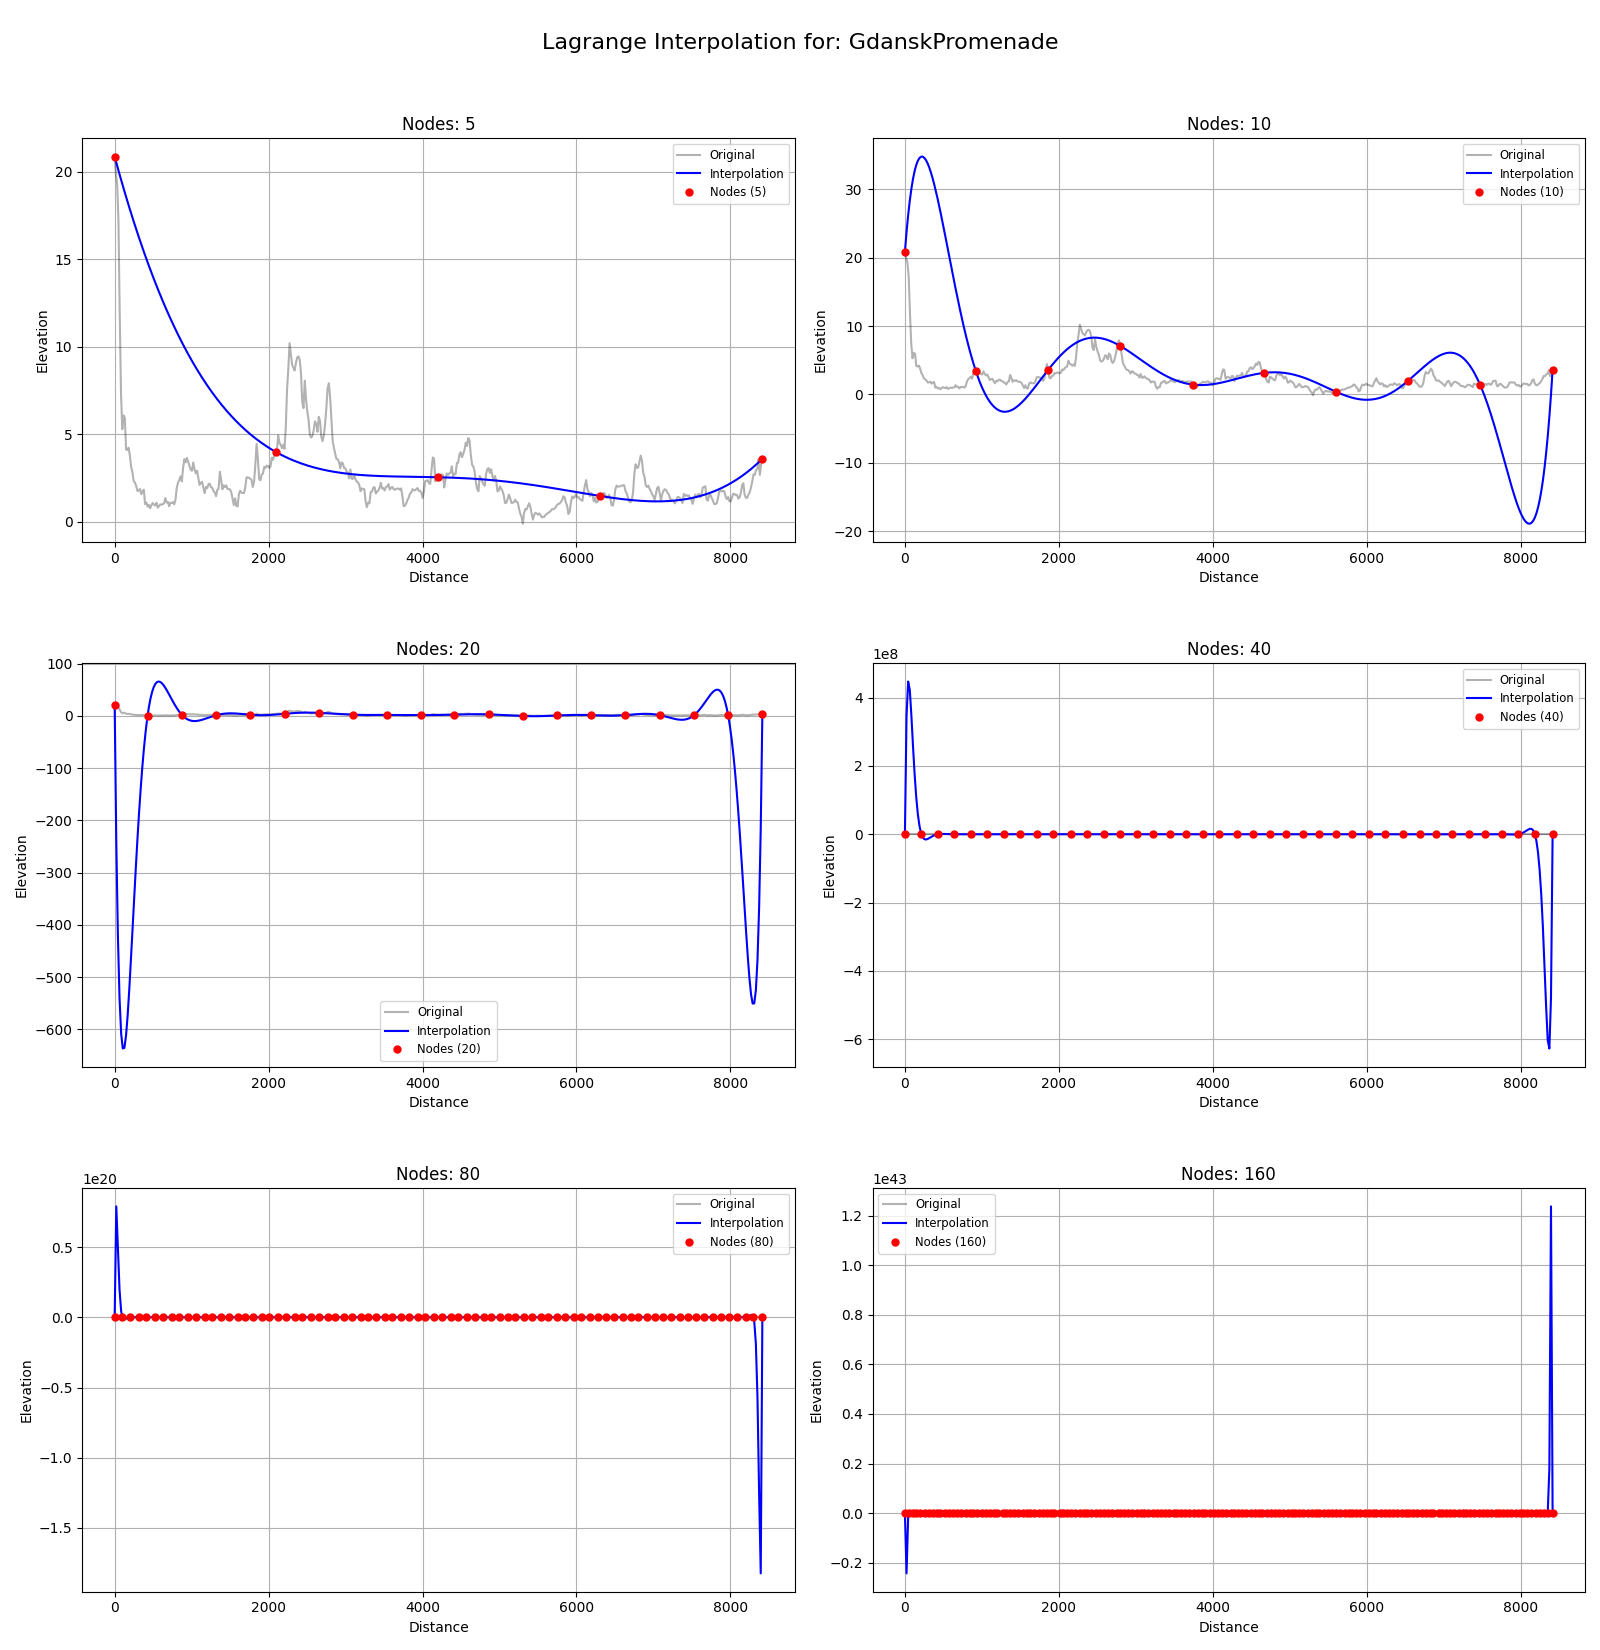
\includegraphics[width=0.8\textwidth]{plots/GdanskPromenade_Lagrange_basic.png}
    \caption{Interpolacja Lagrange'a dla trasy GdanskPromenade (różne liczby węzłów)}
    \label{fig:promenade_lagrange}
\end{figure}
\textbf{Interpretacja (Rysunek \ref{fig:promenade_lagrange}):} 
\begin{itemize}
    \item \textbf{5 węzły:}
    \item \textbf{10 węzłów:}
    \item \textbf{20 węzłów:}
    \item \textbf{40 węzły:} 
    \item \textbf{80 węzły:} 
    \item \textbf{160 węzłów:} 
\end{itemize}

\subsection{Trasa: Hel}
\begin{figure}[H]
    \centering
    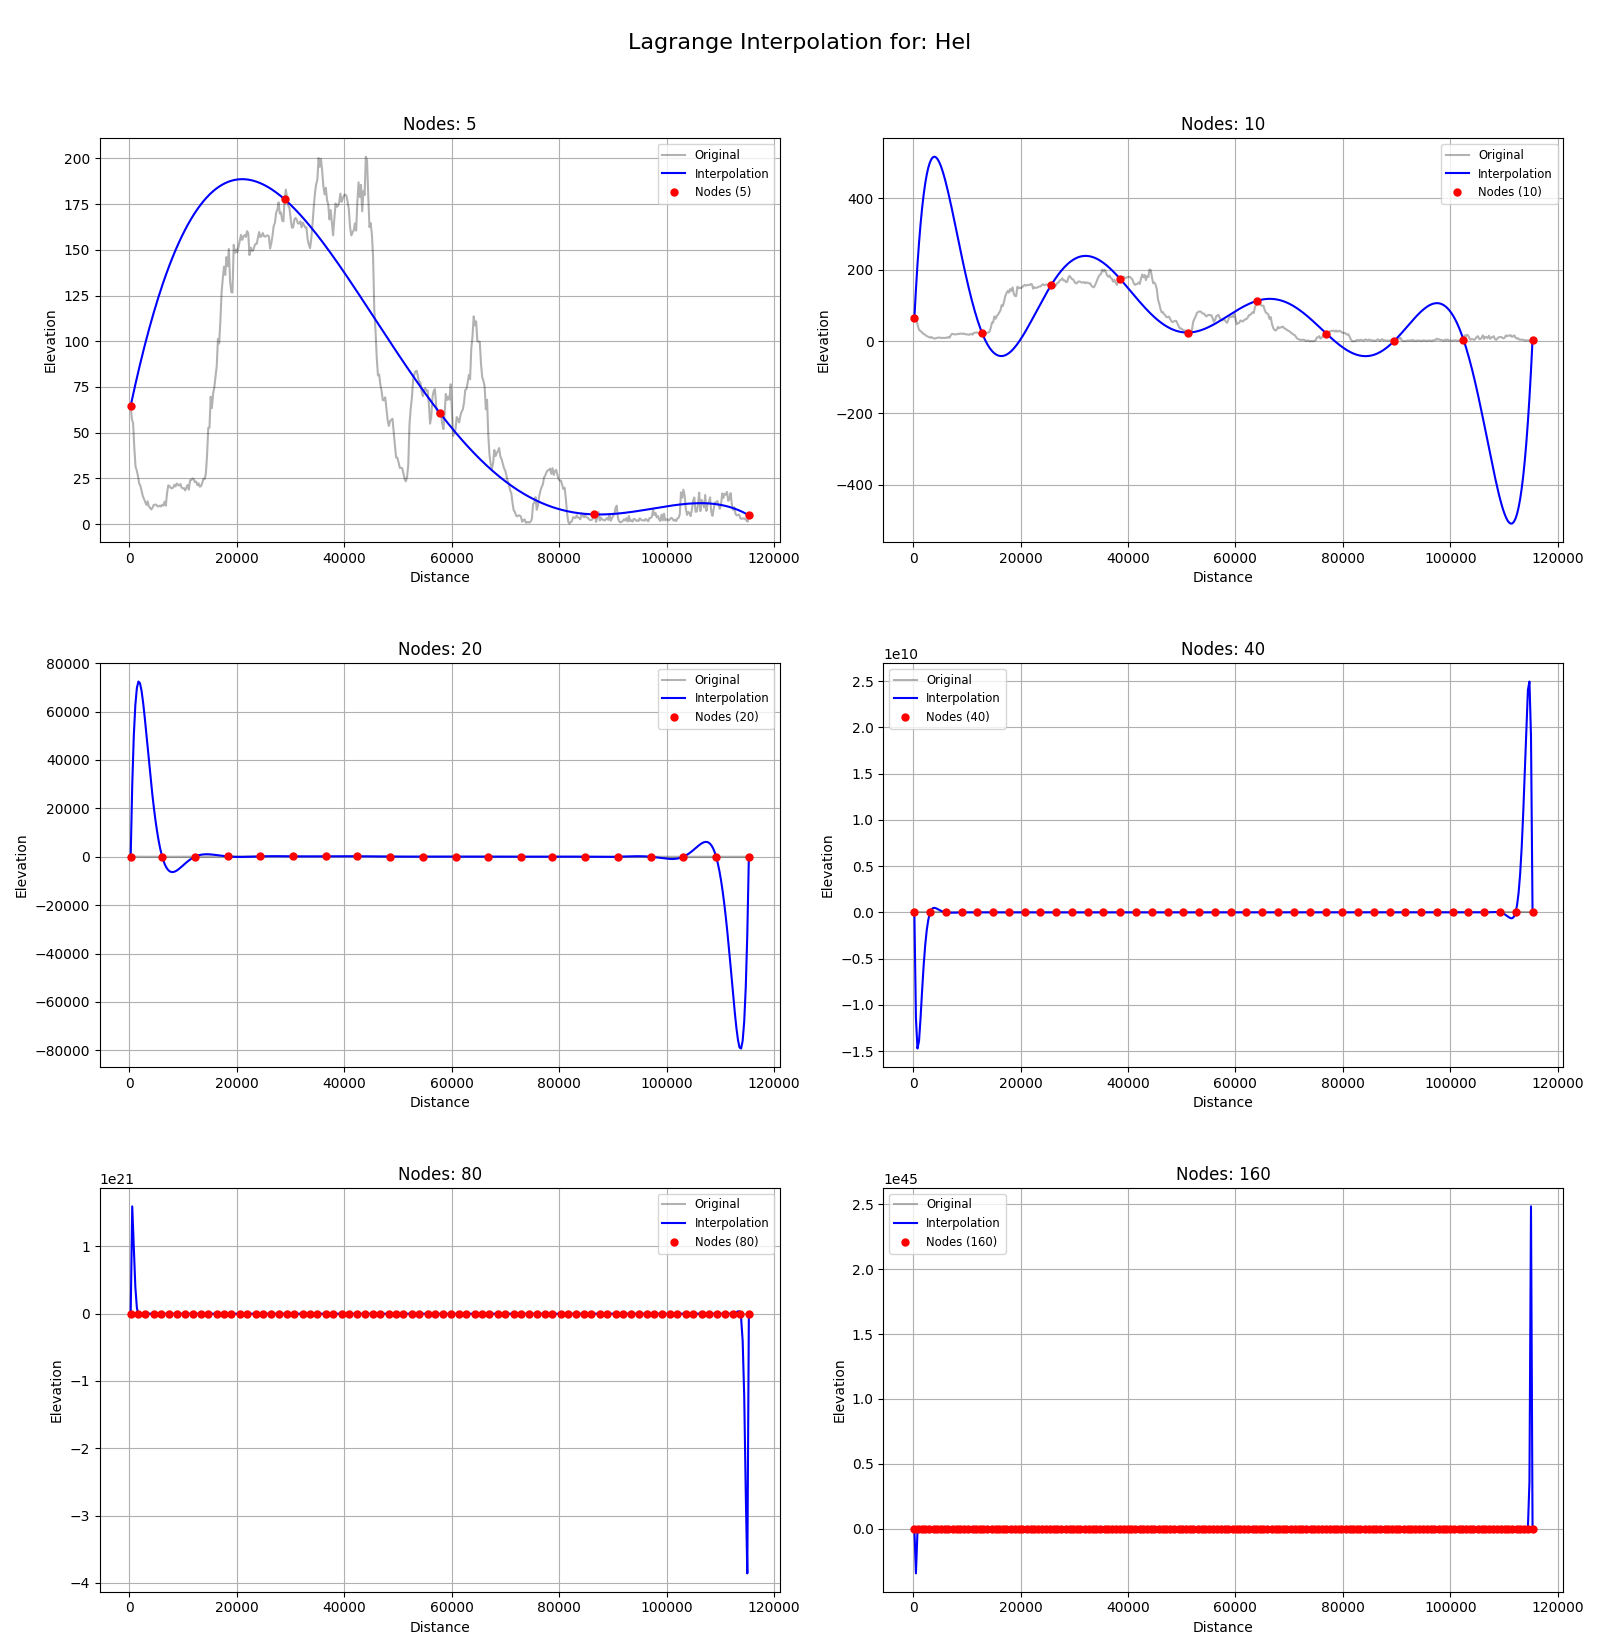
\includegraphics[width=0.8\textwidth]{plots/Hel_Lagrange_basic.png}
    \caption{Interpolacja Lagrange'a dla trasy Hel (różne liczby węzłów)}
    \label{fig:hel_lagrange}
\end{figure}
\textbf{Interpretacja (Rysunek \ref{fig:hel_lagrange}):} 
\begin{itemize}
    \item \textbf{5 węzły:} 
    \item \textbf{10 węzłów:} 
    \item \textbf{20 węzłów:} 
    \item \textbf{40 węzły:} 
    \item \textbf{80 węzły:} 
    \item \textbf{160 węzłów:} 
\end{itemize}

\section{Analiza podstawowa interpolacji funkcjami sklejanymi}
\subsection{Trasa: GdanskPromenade}
\begin{figure}[H]
    \centering
    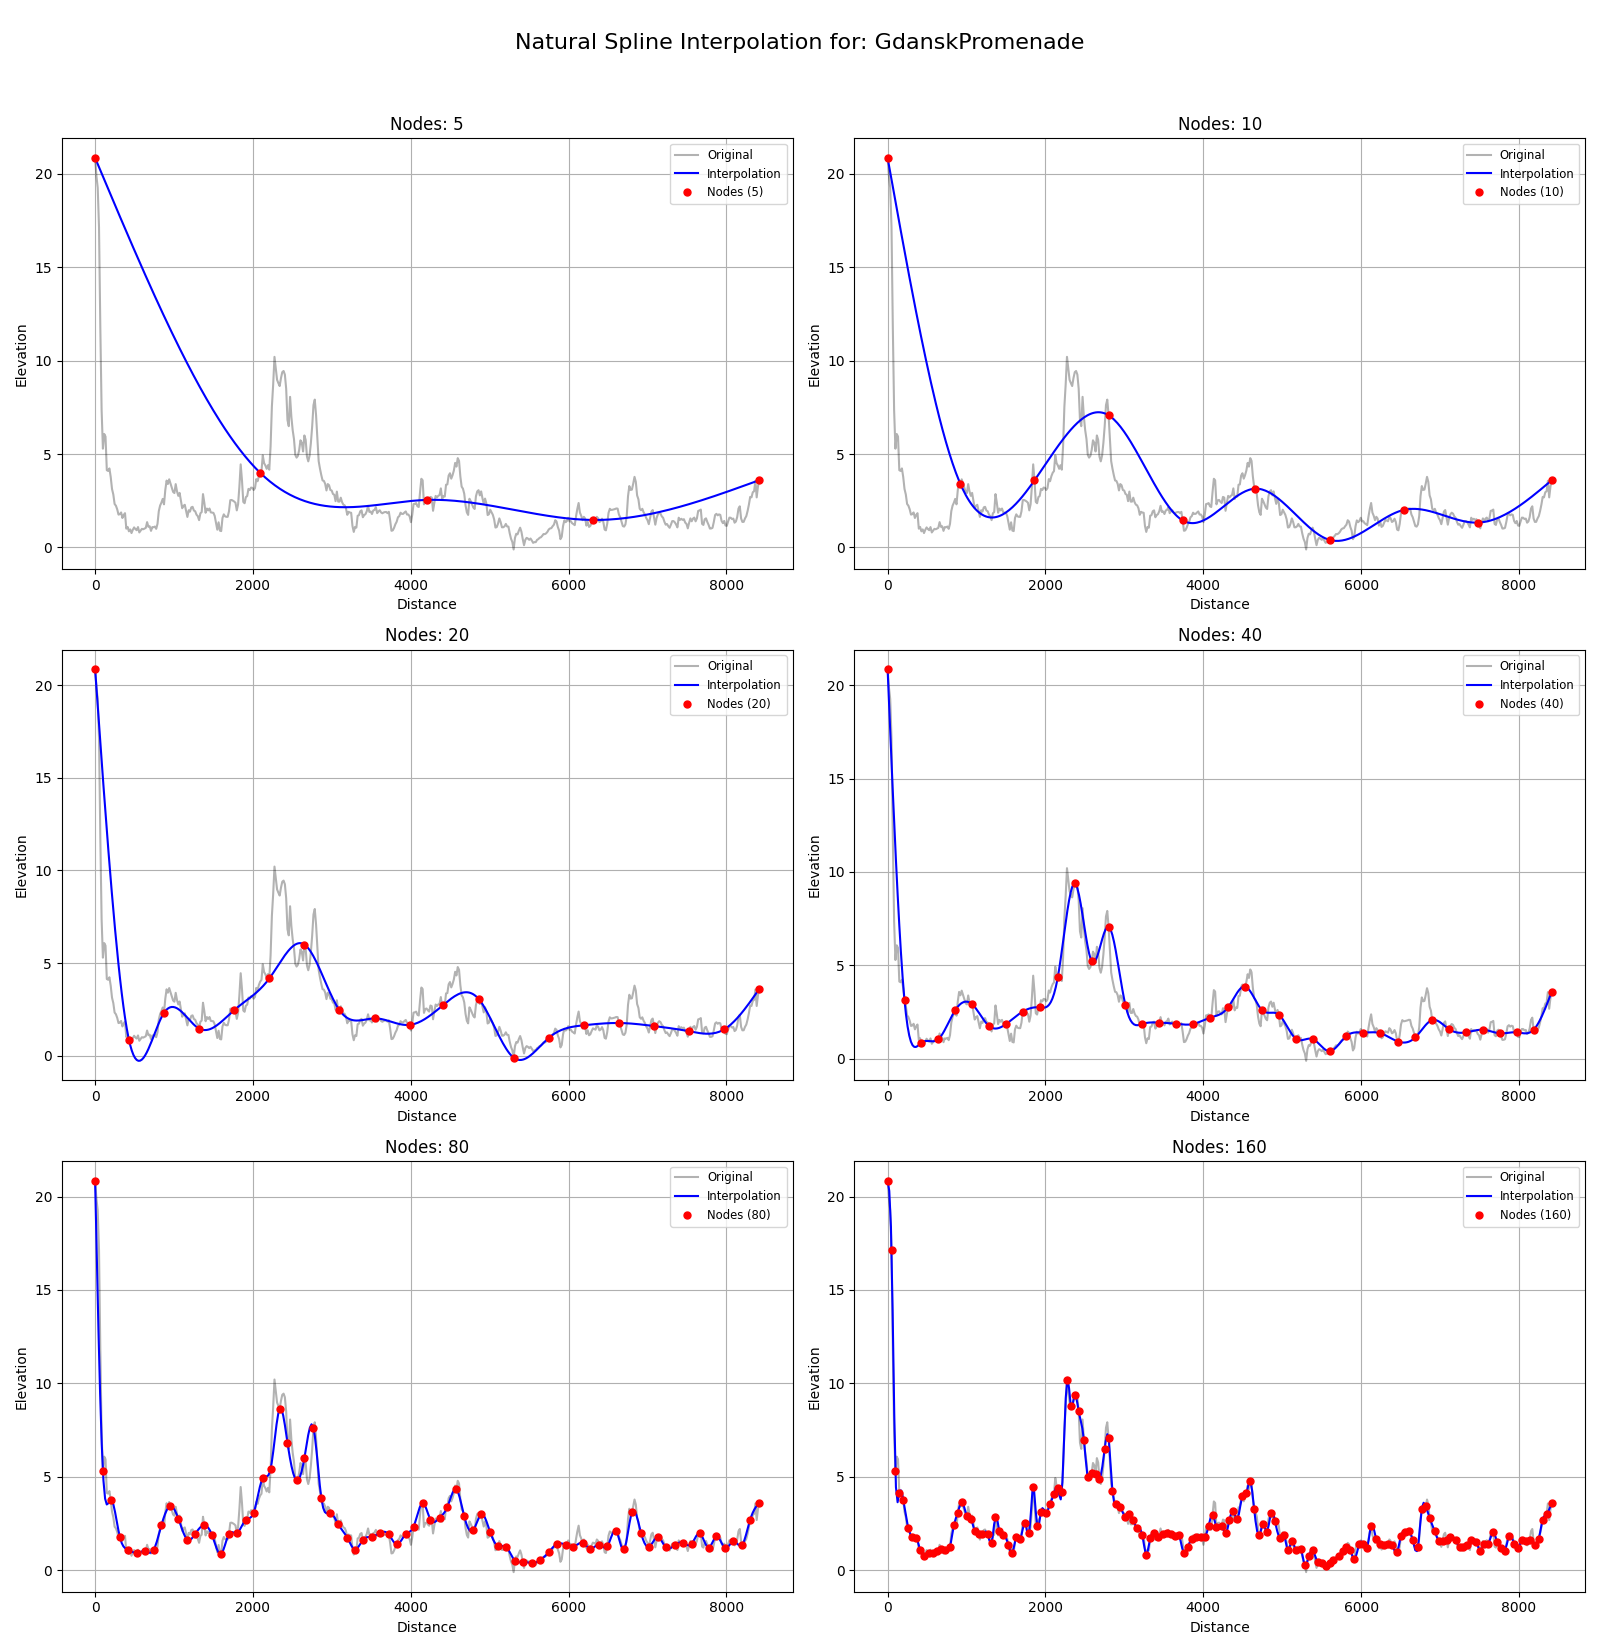
\includegraphics[width=0.8\textwidth]{plots/GdanskPromenade_Spline_basic.png}
    \caption{Interpolacja splajnami kubicznymi dla trasy GdanskPromenade (różne liczby węzłów)}
    \label{fig:promenade_splajny}
\end{figure}
\textbf{Interpretacja (Rysunek \ref{fig:promenade_splajny}):} 
\begin{itemize}
    \item \textbf{5 węzły:}
    \item \textbf{10 węzłów:}
    \item \textbf{20 węzłów:}
    \item \textbf{40 węzły:} 
    \item \textbf{80 węzły:} 
    \item \textbf{160 węzłów:} 
\end{itemize}

\subsection{Trasa: Hel}
\begin{figure}[H]
    \centering
    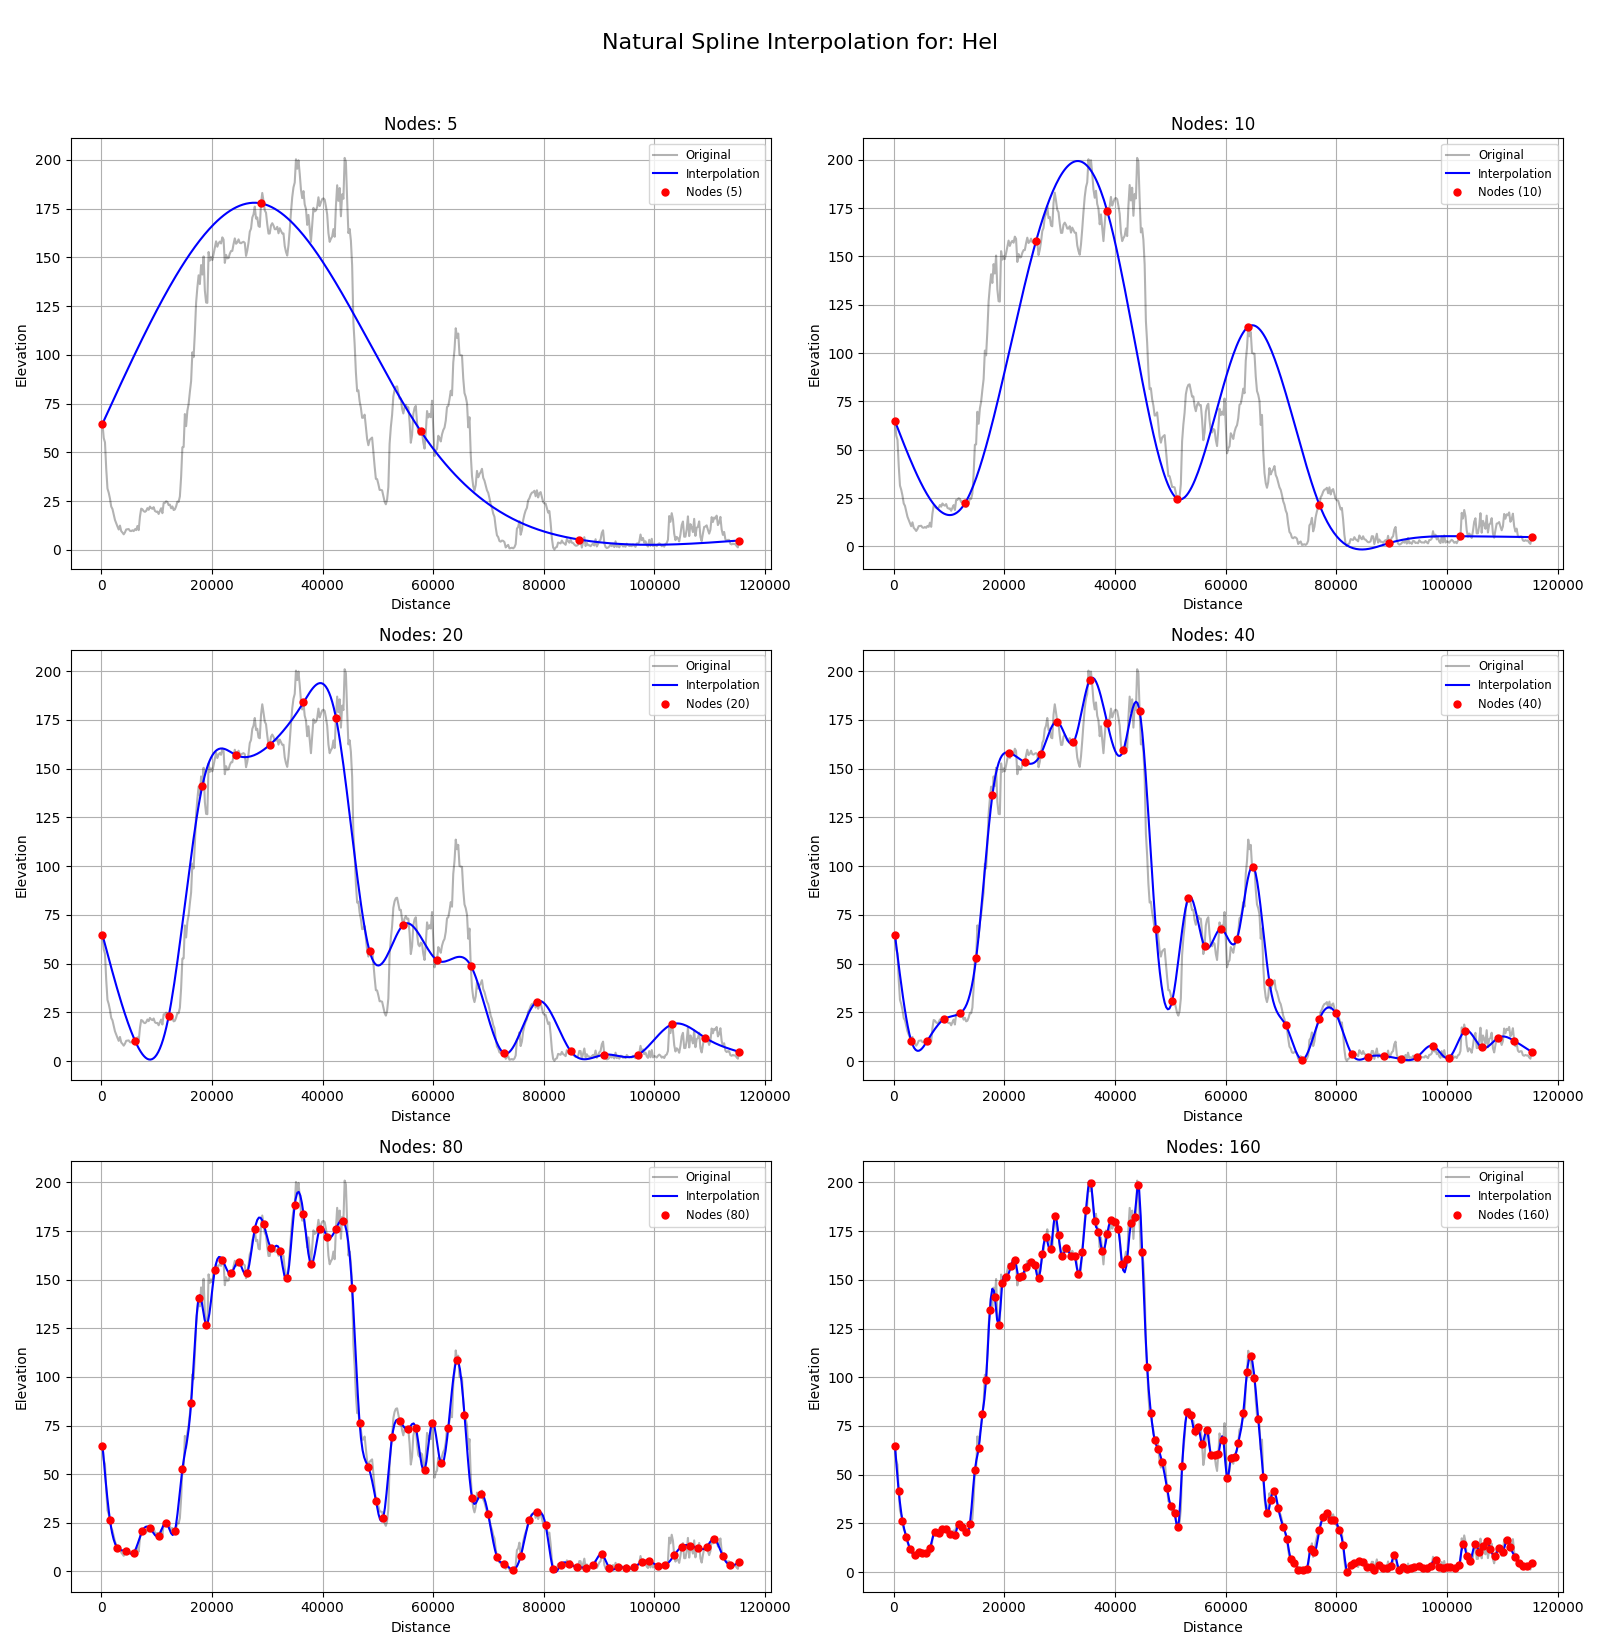
\includegraphics[width=0.8\textwidth]{plots/Hel_Spline_basic.png}
    \caption{Interpolacja splajnami kubicznymi dla trasy Hel (różne liczby węzłów)}
    \label{fig:hej_splajny}
\end{figure}
\textbf{Interpretacja (Rysunek \ref{fig:hej_splajny}):} 
\begin{itemize}
    \item \textbf{5 węzły:}
    \item \textbf{10 węzłów:}
    \item \textbf{20 węzłów:}
    \item \textbf{40 węzły:} 
    \item \textbf{80 węzły:} 
    \item \textbf{160 węzłów:} 
\end{itemize}

\section{Analiza dodatkowa}
\subsection{Wpływ rozmieszczenia węzłów (węzły Czebyszewa)}
\begin{figure}[H]
    \centering
    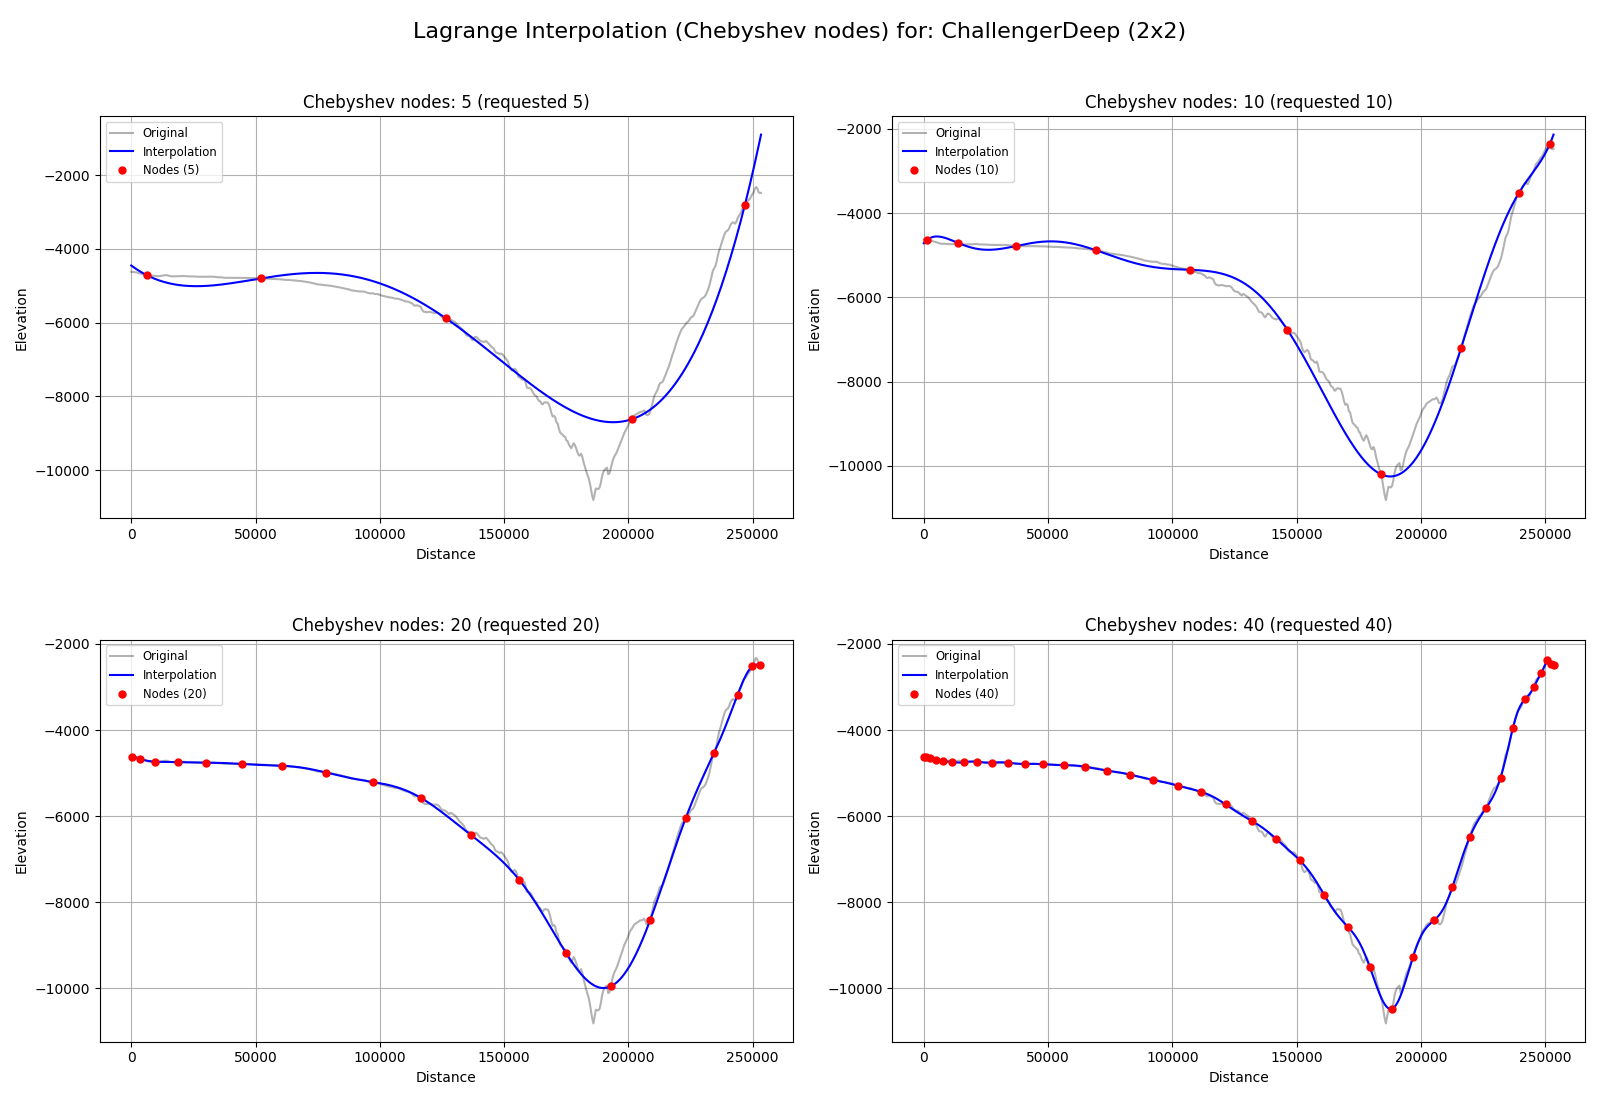
\includegraphics[width=0.8\textwidth]{plots/ChallengerDeep_Lagrange_Chebyshev_2x2.png}
    \caption{Interpolacja Lagrange'a z węzłami Czebyszewa dla trasy ChallengerDeep}
    \label{fig:challengerdeep_chebyshev}
\end{figure}
\textbf{Interpretacja (Rysunek \ref{fig:challengerdeep_chebyshev}):} 
\begin{itemize}
    \item \textbf{5 węzły:}
    \item \textbf{10 węzłów:}
    \item \textbf{20 węzłów:}
    \item \textbf{40 węzły:} 
    \item \textbf{80 węzły:} 
    \item \textbf{160 węzłów:} 
\end{itemize}

\subsection{Trasa o wielu wzniesieniach}
\begin{figure}[H]
    \centering
    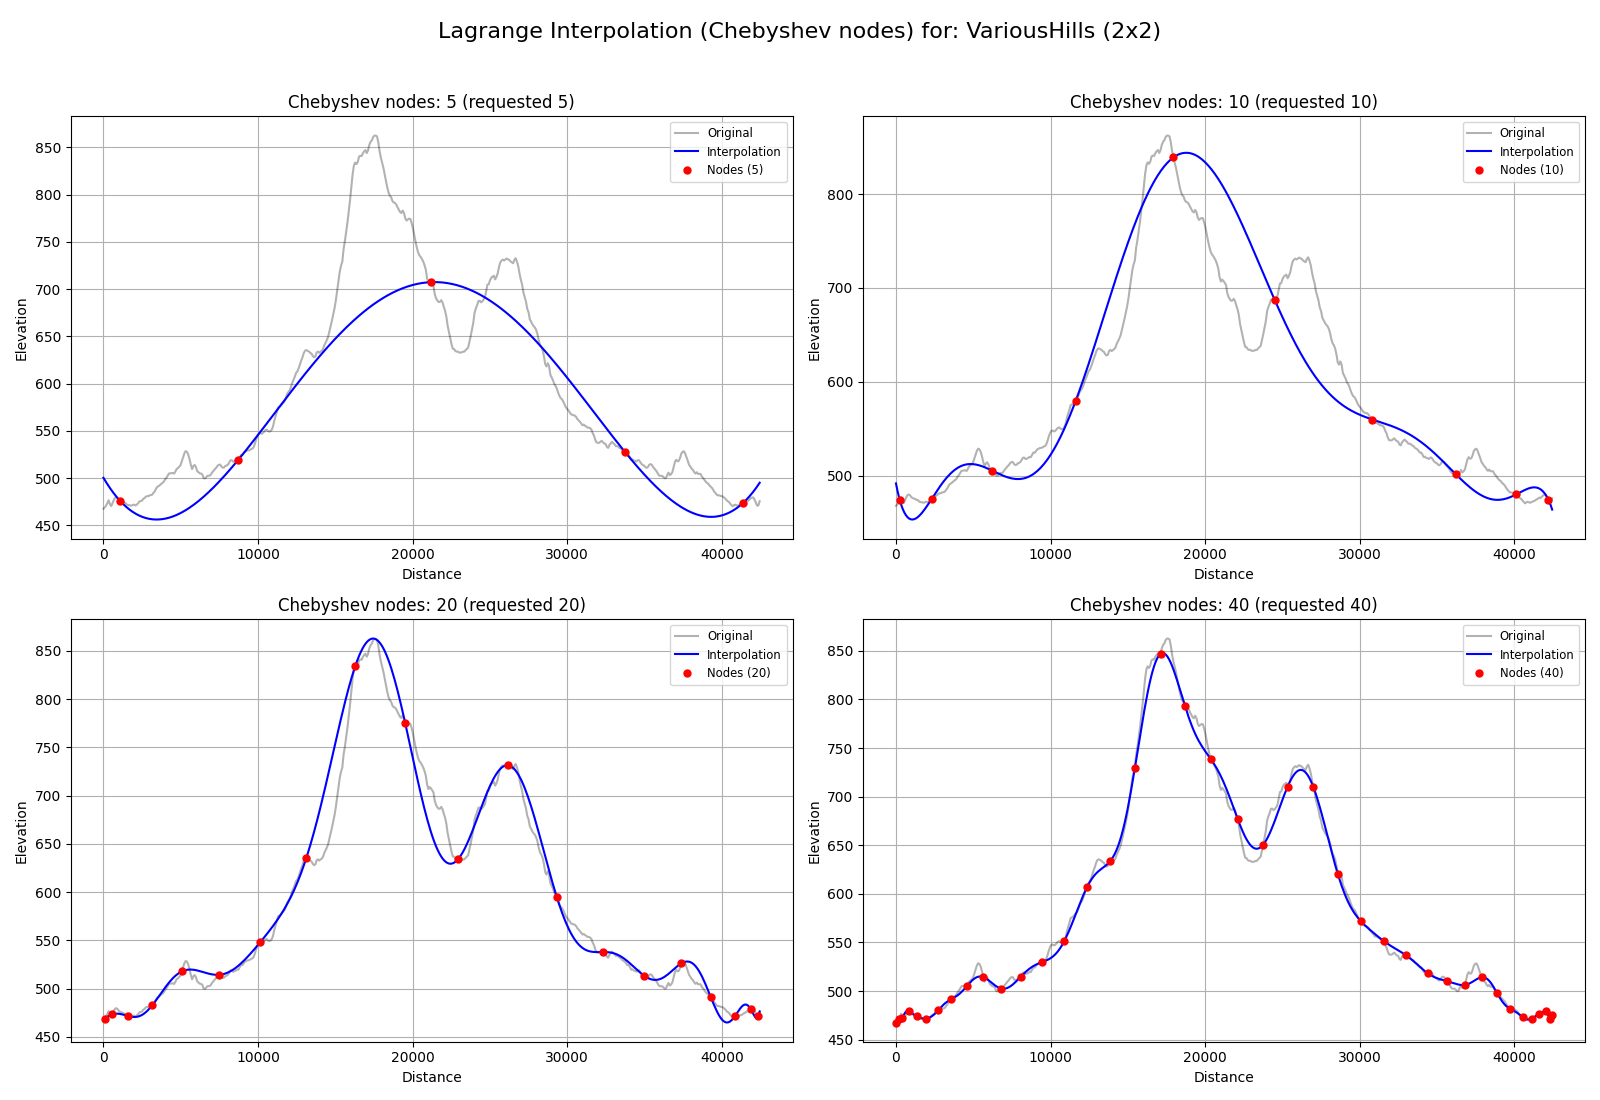
\includegraphics[width=0.8\textwidth]{plots/VariousHills_Lagrange_Chebyshev_2x2.png}
    \caption{Interpolacja Lagrange'a z węzłami Czebyszewa dla trasy VariousHills}
    \label{fig:wiele_wzniesien}
\end{figure}
\textbf{Interpretacja (Rysunek \ref{fig:wiele_wzniesien}):} 
\begin{itemize}
    \item \textbf{5 węzły:}
    \item \textbf{10 węzłów:}
    \item \textbf{20 węzłów:}
    \item \textbf{40 węzły:} 
    \item \textbf{80 węzły:} 
    \item \textbf{160 węzłów:} 
\end{itemize}

\newpage
\section{Interpretacja wyników}
\begin{itemize}
    \item Zwiększanie liczby węzłów w interpolacji Lagrange'a prowadzi do poprawy dokładności tylko do pewnego momentu; dla dużej liczby węzłów pojawia się efekt Rungego (oscylacje na krańcach przedziału).
    \item Rozmieszczenie węzłów według Czebyszewa poprawia stabilność interpolacji wielomianowej.
    \item Interpolacja splajnami kubicznymi jest stabilna nawet dla większej liczby węzłów i dobrze odwzorowuje przebieg trasy.
    \item Charakter trasy (liczba i stromość wzniesień) wpływa na trudność interpolacji -- trasy o gwałtownych zmianach wysokości są trudniejsze do aproksymacji.
\end{itemize}

\section{Podsumowanie}
Refactor!!!
\label{sec:podsumowanie}
Przeprowadzona analiza podstawowa wykazała znaczące różnice w przydatności obu metod do aproksymacji profilu wysokościowego.

\textbf{Interpolacja wielomianem Lagrange'a} okazała się metodą wysoce niestabilną, szczególnie przy większej liczbie równoodległych węzłów interpolacyjnych (16 i więcej w naszych testach). Zjawisko Rungego prowadzi do powstawania dużych, nierealistycznych oscylacji, które całkowicie uniemożliwiają sensowną aproksymację profilu. Metoda ta może być brana pod uwagę jedynie przy bardzo małej liczbie węzłów (np. do około 8) i dla stosunkowo gładkich profili, jednak nawet wtedy jej użyteczność jest ograniczona. Przeskalowanie dziedziny poprawia stabilność numeryczną obliczeń, ale nie eliminuje fundamentalnego problemu oscylacji przy równoodległych węzłach. Jak wykazano w analizie dodatkowej (Sekcja \ref{sec:analiza_dodatkowa}), zastosowanie węzłów Czebyszewa może znacząco zredukować te oscylacje, poprawiając wyniki dla większej liczby węzłów, choć metoda ta nadal pozostaje generalnie mniej stabilna i daje mniej gładkie wyniki niż funkcje sklejane.

\textbf{Interpolacja naturalnymi funkcjami sklejanymi trzeciego stopnia} wykazała się znacznie lepszymi właściwościami. Jest to metoda stabilna, która dostarcza gładkich i wizualnie poprawnych aproksymacji, niezależnie od liczby użytych węzłów (w testowanym zakresie od 4 do 128). Wraz ze wzrostem liczby węzłów, jakość dopasowania systematycznie rośnie, bez wprowadzania niepożądanych artefaktów. Funkcje sklejane dobrze radzą sobie zarówno z profilami gładkimi, jak i bardziej nieregularnymi.

Oceniając działanie zaimplementowanych algorytmów, można stwierdzić, że:
\begin{itemize}
    \item Implementacja interpolacji Lagrange'a poprawnie odzwierciedla matematyczne właściwości tej metody, włączając w to jej podatność na zjawisko Rungego przy węzłach równoodległych oraz poprawę stabilności przy węzłach Czebyszewa. W tym sensie "działa" zgodnie z oczekiwaniami teorii, choć jej praktyczna przydatność do tego zadania jest ograniczona w przypadku węzłów równoodległych.
    \item Implementacja naturalnych funkcji sklejanych trzeciego stopnia działa bardzo dobrze i efektywnie realizuje zadanie aproksymacji profilu wysokościowego.
\end{itemize}

Zdecydowanie rekomendowaną metodą do aproksymacji profili wysokościowych jest interpolacja funkcjami sklejanymi trzeciego stopnia, ze względu na jej stabilność, gładkość wyników i odporność na problemy występujące w interpolacji wielomianowej wysokiego stopnia. Interpolacja Lagrange'a, nawet z węzłami Czebyszewa, powinna być stosowana z ostrożnością i świadomością potencjalnych problemów z oscylacjami.

\end{document}
